%%%%%%%%%%%%%%%%%%%%%%%%%%%%%%%%%%%%%%%%%%%%%%%%%%%%%%%%%%%%%
%% Begin exercise %%
%%%%%%%%%%%%%%%%%%%%%%%%%%%%%%%%%%%%%%%%%%%%%%%%%%%%%%%%%%%%%
\ex{Semiconductor properties}


%%%%%%%%%%%%%%%%%%%%%%%%%%%%%%%%%%%%%%%%%%%%%%%%%%%%%%%%%%%%%
%% Task 1 %%
%%%%%%%%%%%%%%%%%%%%%%%%%%%%%%%%%%%%%%%%%%%%%%%%%%%%%%%%%%%%%

\task{Properties of germanium as semiconductor}

The following problems explore fundamental semiconductor properties of germanium. 
Starting with atomic concentration and intrinsic resistivity, the tasks gradually introduce doping effects 
and compare the electrical behavior of intrinsic and extrinsic materials under simplified assumptions. Take the values from \autoref{table:ex01_germanium_values}.

\begin{table}[ht]
    \centering  % Zentriert die Tabelle
    \begin{tabular}{ll}
        \toprule
        Intrinsic concentration $n_\mathrm{i}$: &  $\SI{2.5 \cdot 10^{13}}{1\per{\cubic{\centi\meter}}}$\\ 
        Mobility $\mu_\mathrm{p}$: &  $\SI{1800}{\frac{\square{\centi\meter}}{\volt\second}}$ \\ 
        Mobility $\mu_\mathrm{n}$: &  $\SI{3800}{\frac{\square{\centi\meter}}{\volt\second}}$ \\ 
        Atomic weight $a_\mathrm{ger}$: &  $\SI{72.6}{\gram\per\mole}$ \\
        Material density $D_\mathrm{ger}$: &  $\SI{5.32}{\gram\per{\cubic{\centi\meter}}}$ \\ 
        \bottomrule
    \end{tabular}
    \caption{key figures of germanium at $\SI{300}{\kelvin}$.}  % Beschriftung der Tabelle
    \label{table:ex01_germanium_values}
\end{table}


\subtask{Using Avogadro’s number ($N_{Av}=\SI{6.02 \cdot 10{23}}{mol^{-1}}$), calculate the concentration of atoms in germanium.}

\begin{solutionblock}
    A quantity of any substance equal to its molecular weight in grams is a mole.
    So the concentration is calculated by
    \begin{equation}
        C_{Ger} = \frac{N_\mathrm{Av}}{a_\mathrm{ger}} \cdot D_\mathrm{ger}
        =\frac{\SI{6.02 \cdot 10{23}}{mol^{-1}}}{\SI{72.6}{\gram\per\mole}} \cdot \SI{5.32}{\gram\per{\cubic{\centi\meter}}}
        = \SI{4.41 \cdot 10^{22}}{atoms\per{\cubic{\centi\meter}}}.
    \end{equation}
\end{solutionblock}

\subtask{Calculate the resistivity of intrinsic germanium at $\SI{300}{\kelvin}$.}

\begin{solutionblock}
    Using the equation $n=p=n_\mathrm{i}$ the conductivity of the intrinsic germanium is calculated by
    \begin{equation}
        \begin{aligned}
            \sigma  &= n_\mathrm{i}q(\mu_n+\mu_p) = \SI{2.5 \cdot 10^{13}}{1\per{\cubic{\centi\meter}}} \cdot \SI{1.60 \cdot 10^{-19}}{\coulomb}
            \cdot \left( \SI{3800}{\square{\centi\meter}\per{\volt\second}} + \SI{1800}{\square{\centi\meter}\per{\volt\second}} \right) \\
            &= \SI{0.00224}{\frac{1}{\ohm\centi\meter}}.
    \end{aligned}        
    \end{equation}
    The resistivity results by the reciprocal value:
    \begin{equation}
        \rho = \frac{1}{\sigma} = \frac{1}{\SI{0.00224}{1\per{\ohm\centi\meter}}}= \SI{44.6}{\ohm\centi\meter}.
    \end{equation}    
\end{solutionblock}


\subtask{If a donor-type impurity is added to the extent of 1 part in $10^8$ germanium atoms, find the resistivity.}

\begin{solutionblock}
    If there is 1 donor atom per $10^8$ germanium atoms, then $N_\mathrm{D}= \SI{4.41 \cdot 10^{14}}{1\per{\cubic{\centi\meter}}}$.
    Using the fact $n \approx N_\mathrm{D}$ leads to:
    \begin{equation}
            p  = \frac{n_\mathrm{i}^2}{N_\mathrm{D}}
            = \frac{\left({\SI{2.5 \cdot 10^{13}}{1\per{\cubic{\centi\meter}}}}\right)^2}{\SI{4.41 \cdot 10^{14}}{1\per{\cubic{\centi\meter}}}}
            = \SI{1.42 \cdot 10^{12}}{holes\per{\cubic{\centi\meter}}}.
    \end{equation}
    Since $n \gg p$, we can neglect $p$ in calculating the conductivity. This leads to:
    \begin{equation}
        \sigma = nq\mu_n = \SI{4.41 \cdot 10^{14}}{1\per{\cubic{\centi\meter}}} \cdot \SI{1.60 \cdot 10^{-19}}{\coulomb}
        \cdot \SI{3800}{\square{\centi\meter}\per{\volt\second}} = \SI{0.268}{\frac{1}{\ohm\centi\meter}}.
    \end{equation}
    The resistivity results by the reciprocal value:
    \begin{equation}
        \rho = \frac{1}{\sigma} = \frac{1}{\SI{0.268}{1\per{\ohm\centi\meter}}}= \SI{3.72}{\ohm\centi\meter}.
    \end{equation} 
\end{solutionblock}


\subtask{If germanium were a monovalent metal, find the ratio of its conductivity to that of the n-type semiconductor in previous subtask.}

\begin{solutionblock}
    If each atom contributed one free electron to the material the number of free electrons are $n  = 4.41 \cdot 10^{22}$.
    This leads to:
    \begin{equation}
        \sigma = nq\mu_\mathrm{n} = \SI{4.41 \cdot 10^{22}}{1\per{\cubic{\centi\meter}}} \cdot \SI{1.60 \cdot 10^{-19}}{\coulomb}
        \cdot \SI{3800}{\square{\centi\meter}\per{\volt\second}} = \SI{2.58 \cdot 10^{7}}{\frac{1}{\ohm\centi\meter}}.
    \end{equation}
    The ratio yields:
    \begin{equation}
        \frac{\sigma_{metal}}{\sigma_\mathrm{semi}}= \frac{ \SI{2.58 \cdot 10^{7}}{\frac{1}{\ohm\cubic{\centi\meter}}}}{\SI{0.268}{1\per{\ohm\centi\meter}}}
        \approx 10^8.
    \end{equation}

\end{solutionblock}




%%%%%%%%%%%%%%%%%%%%%%%%%%%%%%%%%%%%%%%%%%%%%%%%%%%%%%%%%%%%%
%% Task 2 %%
%%%%%%%%%%%%%%%%%%%%%%%%%%%%%%%%%%%%%%%%%%%%%%%%%%%%%%%%%%%%%

\task{Energy level and silicon semiconductor behaviour.} 

\subtask{Calculate the frequency of revolution for an electron in the ground state of hydrogen. For comparison, find the
frequency emitted when an electron with the mass $m_\mathrm{e}=\SI{9.11 \cdot 10^{-31}}{\kilo\gram}$ of falls from the state $n=2$ to the ground state $n=1$. 
Take in account, that $W_\mathrm{kin}(n)\propto \frac{1}{n^2}$ and the ground state orbit $r$ corresponds to $\SI{0.0529}{\nano\meter}$.}

\begin{solutionblock}
    The kinetic energy of this electron for ground state is calculated by
    \begin{equation}
        W_\mathrm{kin}= \frac{1}{2} m_\mathrm{e}v^2 = \frac{1}{2} m_\mathrm{e} r \omega^2.
        \label{eq:Wkinmech}
    \end{equation}
    If the electron with the mass $m_\mathrm{e}$ orbits a proton in a circular path with radius $r$ and speed $v$, the centrifugal force 
    (from circular motion) is balanced by the electrostatic attraction (Coulomb force) between the electron and the proton.
    This balance leads to the equation:
    \begin{equation}
        m_\mathrm{e} r \omega^2 = \frac{{q_\mathrm{e}}^2}{4\pi\epsilon_0}
        \label{eq:Wkinelec}
    \end{equation}   
    Using \eqref{eq:Wkinmech} and \eqref{eq:Wkinelec} leads to 
    \begin{equation}
        W_\mathrm{kin} = \frac{1}{8\pi\epsilon_0} \cdot \frac{{q_\mathrm{e}}^2}{r n^2}
        =\frac{1}{8\pi \cdot \SI{8.854 \cdot 10^{-12}}{\farad\per\meter}} \cdot \frac{({\SI{1.60 \cdot 10^{-19}}{\coulomb}})^2}{\SI{0.0529}{\nano\meter}} 
        =  \SI{2.17 \cdot 10^{-18}}{\joule}
    \end{equation}   
    Solving \eqref{eq:Wkinmech} for $\omega$ yields
    \begin{equation}
        \begin{aligned}
            \omega &= \sqrt{\frac{2 \cdot W_\mathrm{kin}}{ m_\mathrm{e} r}} = \sqrt{\frac{2 \cdot \SI{2.17 \cdot 10^{-18}}{\joule}}{\SI{9.11 \cdot 10^{-31}}{\kilo\gram} \cdot \SI{0.0529}{\nano\meter}}}
            = \SI{3 \cdot 10^{11}}{1\per\second}. \\
            f& = \SI{47.8}{\giga\hertz}.
        \end{aligned}
    \end{equation}
    The total energy for ground state is calculated by
    \begin{equation}
        W_\mathrm{n=1} = -\frac{{q_\mathrm{e}}^2}{8\pi\epsilon_0 r}=
        = - \frac{{\SI{1.60 \cdot 10^{-19}}{\coulomb}}^2}{8\pi \cdot \SI{8.854 \cdot 10^{-12}}{\farad\per\meter} \cdot \SI{0.0529}{\nano\meter} }
        =  \SI{-2.17 \cdot 10^{-18}}{\joule}
    \end{equation}
    The energy difference a transition from $n=2$ to $n=1$ is calculated by
    \begin{equation}
        \Delta W= W_\mathrm{n=1} \cdot \left(\frac{1}{2^2} -1 \right)=\SI{-2.17 \cdot 10^{-18}}{\joule} \cdot (-0.75) = \SI{1.63 \cdot 10^{-18}}{\joule}
    \end{equation}
    This corresponds to a frequency of
    \begin{equation}
        f = \frac{\Delta W} {h}=\frac{\SI{1.63 \cdot 10^{-18}}{\joule}} {\SI{6.63 \cdot 10^{-34}}{\joule\per\second}} = \SI{2.5 \cdot 10^{15}}{\hertz}
    \end{equation}       
\end{solutionblock}




\subtask{Find the room-temperature resistivity of an n-type silicon doped with $10^{16}$ phosphorus $\si{atoms\per \cubic{\centi\meter}}$.}

\begin{solutionblock}
    At room temperature we assume that all donors are ionized. 
    This leads to:
    \begin{equation}
        n \approx N_\mathrm{D} = \SI{10^{16}}{1\per{\cubic{\centi\meter}}}.
    \end{equation}
    The conductivity is calculated by
    \begin{equation}
        \sigma = nq\mu_n = \SI{10^{16}}{1\per{\cubic{\centi\meter}}} \cdot \SI{1.60 \cdot 10^{-19}}{\coulomb}
        \cdot \SI{1300}{\square{\centi\meter}\per{\volt\second}} = \SI{20.8}{\frac{1}{\ohm\centi\meter}}.
    \end{equation}
    The resistivity results by the reciprocal value:
    \begin{equation}
        \rho = \frac{1}{\sigma} = \frac{1}{\SI{20.8}{{\ohm\centi\meter}^{-1}}}= \SI{0.48}{\ohm\centi\meter}.
    \end{equation} 
\end{solutionblock}


\subtask{A sample of Si is doped with $10^{16}$ phosphorus $\si{atoms\per \cubic{\centi\meter}}$. 
Find the Hall voltage in a sample with $l_\mathrm{w} = \SI{500}{\micro\meter}$, $A = \SI{2.5 \cdot 10^{-3}}{\square\centi\meter}$, $I = \SI{1}{\milli\ampere}$, 
and $B_\mathrm{z} =  \SI{10^{-4}}{\weber\per\square\centi\meter}$.}

\begin{solutionblock}
    The Hall coefficient is calculated by
    \begin{equation}
        R_\mathrm{H} = \frac{1}{qn} = \frac{1}{\SI{1.60 \cdot 10^{-19}}{\coulomb} \cdot \SI{10^{16}}{\frac{1}{\cubic{\centi\meter}}}} =  \SI{625}{\cubic{\centi\meter}\per\coulomb}.
    \end{equation}
    The Hall voltage results from
    \begin{equation}
        U_\mathrm{H} = R_\mathrm{H} \frac{I}{A}B_\mathrm{z} l_\mathrm{w} = \SI{625}{\cubic{\centi\meter}\per\coulomb} \frac{\SI{1}{\milli\ampere}}{\SI{2.5 \cdot 10^{-3}}{\square\centi\meter}}
        \SI{10^{-4}}{\weber\per\square\centi\meter} \cdot \SI{500}{\micro\meter} = \SI{-1.25}{\milli\volt}.
    \end{equation}
\end{solutionblock}

\subtask{ Assume that, in an n-type semiconductor at $T = \SI{300}{\kelvin}$, the electron concentration varies linearly from 
 $\SI{10^{18}}{1\per\cubic{\centi\meter}}$ to $\SI{7 \cdot 10^{17}}{1\per\cubic{\centi\meter}}$ over a distance of $\SI{0.1}{\centi\meter}$.
  Calculate the diffusion current density if the electron diffusion coefficient is $D_n = \SI{22.5}{\square\centi\meter\per\second}$.}

\begin{solutionblock}
    The diffusion current density is given by
    \begin{equation}
        \begin{aligned}
            J_\mathrm{n,diff} &= qD_\mathrm{n} \frac{\mathrm{d}n}{\mathrm{d}x} \approx qD_\mathrm{n} \frac{\mathrm{\Delta} n}{\mathrm{\Delta} x} \\
            &= \SI{1.60 \cdot 10^{-19}}{\coulomb} \cdot \SI{22.5}{\square\centi\meter\per\second} \cdot
            \frac{\SI{10^{18}}{\frac{1}{\cubic{\centi\meter}}} - \SI{7 \cdot 10^{17}}{\frac{1}{\cubic{\centi\meter}}}}{\SI{0.1}{\centi\meter}}
            = \SI{10.8}{\ampere\per\square\centi\meter}.
        \end{aligned}
    \end{equation}
\end{solutionblock}

\subtask{Minority carriers (holes) are injected into a homogeneous n-type semiconductor sample at one point.
 An electric field of $\SI{50}{\volt\per{\centi\meter}}$ is applied across the sample,
 and the field moves these minority carriers a distance of $\SI{1}{\centi\meter}$ in $\SI{100}{\micro\second}$.
 Find the drift velocity and the diffusivity of the minority carriers. The temperature is $\SI{300}{\kelvin}$.}
 \begin{solutionblock}
    The drift velocity is simply calculated by the distance traveled per unit time.
    \begin{equation}
        v_\mathrm{p} = \frac{l_\mathrm{d}}{t} = \frac{\SI{1}{\centi\meter}}{\SI{100}{\micro\second}} = \SI{10^4}{\centi\meter\per\second}.
    \end{equation}
    The mobility results from the quotient of drift velocity and the electrical field along parallel to the drift direction.
    \begin{equation}
        \mu_\mathrm{p} = \frac{v_\mathrm{p}}{\vec{E}} = \frac{\SI{10^4}{\centi\meter\per\second}}{\SI{50}{\volt\per{\centi\meter}}}
        = \SI{200}{\frac{\square{\centi\meter}}{\volt\second}}.
    \end{equation}
    This leads to the diffusivity of the minority carriers:
    \begin{equation}
        D_\mathrm{p} = \frac{kT}{q} \mu_\mathrm{p} = \frac{\SI{1.38 \cdot 10^{-19}}{\joule\per\kelvin} \cdot \SI{300}{\kelvin}}
                        {\SI{1.60 \cdot 10^{-19}}{\coulomb}} \cdot \SI{200}{\frac{\square{\centi\meter}}{\volt\second}}
        = \SI{5.18}{\frac{\square{\centi\meter}}{\second}}.
    \end{equation}    
\end{solutionblock}

%%%%%%%%%%%%%%%%%%%%%%%%%%%%%%%%%%%%%%%%%%%%%%%%%%%%%%%%%%%%%
%% Task 3 %%
%%%%%%%%%%%%%%%%%%%%%%%%%%%%%%%%%%%%%%%%%%%%%%%%%%%%%%%%%%%%%

\task{Quality assessment at doping of silicon semiconductor}
    
A silicon semiconductor is to be doped for a specific application. To assess the doping quality, the resistivity of a sample is measured before and after the process.
The assessment is performed at a temperature of $T = \SI{300}{\kelvin}$.
\begin{table}[ht]
    \centering  % Zentriert die Tabelle
    \begin{tabular}{ll}
        \toprule
        Intrinsic concentration $n_\mathrm{i}$: &  $\SI{1.5 \cdot 10^{10}}{\per{\cubic{\centi\meter}}}$\\ 
        Mobility $\mu_\mathrm{p}$: &  $\SI{480}{\frac{\square{\centi\meter}}{\volt\second}}$ \\ 
        Mobility $\mu_\mathrm{n}$: &  $\SI{1350}{\frac{\square{\centi\meter}}{\volt\second}}$ \\ 
        \bottomrule
    \end{tabular}
    \caption{key figures of silicon.}  % Beschriftung der Tabelle
    \label{table:ex01_silicon_values}
\end{table}

\subtask{Calculate the expected resistivity of silicon before doping.}
\begin{solutionblock}
    The number of holes are equal to the numbers of free electrons according $n_0 = p_0 = n_i$. 
    So the total conductivity is calculated by
    \begin{equation}
        \begin{aligned}        
            \sigma &= n_\mathrm{i}q(\mu_\mathrm{p}+\mu_\mathrm{n}) \\
                   &= \SI{1.5 \cdot 10^{10}}{\per{\cubic{\centi\meter}}} \cdot \SI{1.60 \cdot 10^{-19}}{\coulomb} \cdot
                    \left(\SI{480}{\frac{\square{\centi\meter}}{\volt\second}}+\SI{1350}{\frac{\square{\centi\meter}}{\volt\second}}\right)
                    = \SI{4.39 \cdot 10^{-6}}{\frac{1}{\ohm\centi\meter}}.
        \end{aligned}                 
    \end{equation}
    The resistivity results by the reciprocal value:
    \begin{equation}
        \rho = \frac{1}{\sigma} = \frac{1}{\SI{4.39 \cdot 10^{-6}}{{\ohm\centi\meter}^{-1}}}= \SI{2.28 \cdot 10^5}{\ohm\centi\meter}.
    \end{equation}     
\end{solutionblock}


\subtask{Calculate the expected resistivity of silicon at $T = \SI{300}{\kelvin}$ after doping with arsenic impurities 
with concentration $N_d = 2\cdot \SI{10^{16}}{\cubic{\centi\meter}}$.}
\begin{solutionblock}
    The concentration of majority carriers is so large that only they will be considered in the following calculation. 
    With $n_0 \approx N_\mathrm{d}$ the conductivity is calculated by:
    \begin{equation}
        \sigma \approx N_\mathrm{d}q\mu_\mathrm{n}
               \approx  2\cdot \SI{10^{16}}{\cubic{\centi\meter}} \cdot \SI{1.60 \cdot 10^{-19}}{\coulomb} \cdot
                 \SI{1350}{\frac{\square{\centi\meter}}{\volt\second}}
                 = \SI{2.3}{\frac{1}{\ohm\centi\meter}}.
    \end{equation}
    The resistivity results by the reciprocal value:
    \begin{equation}
        \rho = \frac{1}{\sigma} = \frac{1}{\SI{2.3}{{\ohm\cubic{\centi\meter}}^{-1}}}= \SI{0.31}{\ohm\centi\meter}.
    \end{equation}     
\end{solutionblock}





%%%%%%%%%%%%%%%%%%%%%%%%%%%%%%%%%%%%%%%%%%%%%%%%%%%%%%%%%%%%%
%% Task 4 %%
%%%%%%%%%%%%%%%%%%%%%%%%%%%%%%%%%%%%%%%%%%%%%%%%%%%%%%%%%%%%%

\task{Hall sensor for  magnetic field measurement}

A bar of type p silicon, of thickness $d=\SI{0.5}{\milli\meter}$, with impurity concentration $N_a = \SI{10^{14}}{\cubic{\centi\meter}}$, is used as a Hall sensor.
See also \autoref{fig:ex01_hallsensor}.

\begin{figure}[htbp]
    \centering      
    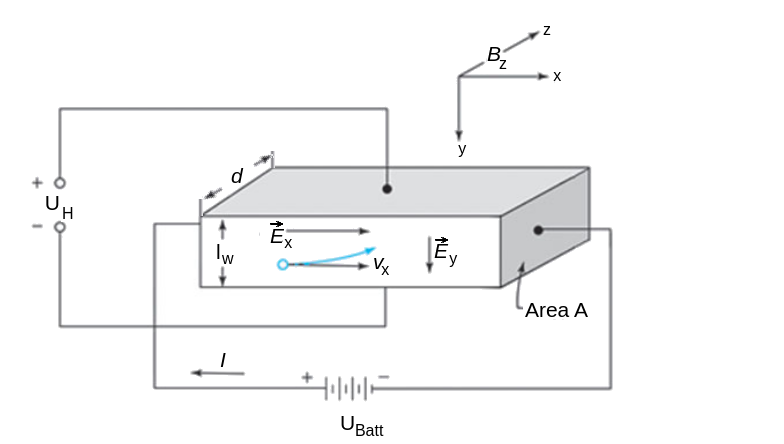
\includegraphics[width=0.5\textwidth]{fig/fig1_ex01_Hall.png}
    \caption{Silicon semiconductor bar as Hall-sensor.}
    \label{fig:ex01_hallsensor}
\end{figure}

\subtask{Calculate the Hall voltage for a probe current of $\SI{100}{\milli\ampere}$ and a magnetic field perpendicular to the plane of $B= \SI{0.1}{\tesla}$.}

\begin{solutionblock}
    The Hall voltage is given by
    \begin{equation}
        U_\mathrm{H} = \vec{E_\mathrm{y}}l_\mathrm{w} \quad \text{and} \quad J = \frac{I}{l_\mathrm{w}d}.
        \label{eq:hall_voltage}
    \end{equation}
    with $l_\mathrm{w}$ corresponds to the width and $d$ to the thickness of the bar. $J$ corresponds to the current density.
    Since $N_\mathrm{a} \gg n_\mathrm{i}$ which leads to $p \approx N_\mathrm{a} \gg n$, so that the current is dominated by holes.
    The electrical field in y-direction results in
    \begin{equation}
        \vec{E_\mathrm{y}}=\frac{J_\mathrm{p}}{qp}B_\mathrm{z}
    \end{equation}
    Using \eqref{eq:hall_voltage} this leads to 
    \begin{equation}
        U_\mathrm{H} = \frac{J_\mathrm{p}}{qp}B_\mathrm{z} l_\mathrm{w} = \frac{I \cdot B_\mathrm{z}}{qpd}
        = \frac{\SI{100}{\milli\ampere} \cdot \SI{0.1}{\tesla}}{\SI{1.60 \cdot 10^{-19}}{\coulomb} \cdot \SI{10^{14}}{\frac{1}{\cubic{\centi\meter}}} \cdot \SI{0.1}{\milli\meter}}
        = \SI{1.25}{\volt} 
    \end{equation} 
\end{solutionblock}    
\vspace{0.5cm}
Remark: This example shows that for magnetic fields with intensities typical of those used in laboratories, the Hall voltage has a relatively high value for electronic
circuits. This does not happen in metals, because the concentration of free electrons $\approx \SI{10^{22}}{\frac{1}{\cubic{\centi\meter}}}$ is much larger than in semiconductors, and thus the
voltage is quite small.